\section{Introduction}
\label{sec:intro}

Reasoning language models such as \dsseven{} and \qweneight{}
\citep{deepseekr1,qwen3,openai_o1} solve hard problems by emitting long chains of
thought, often thousands of tokens per query. Much of this computation is spent
\emph{after} the model has effectively decided on an answer, which makes
\emph{early exit}---halting generation once the answer is settled---an appealing
lever for cutting inference cost \citep{overthinking,dynasor_certaindex}. A
widely used family of methods does this by \emph{probing}: at regular intervals
the partial trajectory is queried for its current answer (e.g., by appending a
short ``\texttt{Final Answer:}'' suffix), and generation is halted once several
probes \emph{agree} \citep{dynasor_certaindex}. The bet is that
\emph{intermediate consensus signals termination}---once the model repeatedly
says the answer is $x$, further reasoning is unlikely to change it. This paper
asks a single question: \textbf{is intermediate agreement a safe signal on which
to stop?}\footnote{We use ``false consensus'' for the phenomenon that
intermediate probe agreement is non-terminal; the term is unrelated to the
social-psychology ``false consensus effect'' \citep{ross1977false}. We study
answer-level early exit (stopping a chain of thought), not token- or layer-level
early exit \citep{graves2016act,schuster2022confident}.}

Our answer is \textbf{no}, and the reason is not a badly tuned threshold---it is
the signal itself. Intermediate consensus forms \emph{while the answer is still
moving}: on a frozen replay, stopping on consensus destroys a
correct-in-the-end answer roughly $\mathbf{35}$ times more often than it rescues
a wrong one (Section~\ref{sec:mechanism}). This is an \emph{accuracy tax} that is
a property of the reasoning trajectory, not of how one probes it, so no threshold
on the agreement signal can escape it. We make the claim hard to dismiss as
``you did not tune it well'' by searching the space exhaustively under
commitment: on frozen trajectories from two models and three benchmarks we run a
\emph{preregistered} sweep of a seven-dimensional consensus-rule schema
($17{,}712$ rules) with problem-grouped splits and acceptance gates fixed in
advance (Sections~\ref{sec:method}--\ref{sec:results}). The outcome does not
depend on any single fragile estimate: \textbf{every one of the $17{,}712$ rules
loses accuracy in the worst case; none reaches break-even.} The frontier
reproduces on a held-out test split ($r{=}0.96$) and on unseen models at
$4\times$ the scale and a different architecture (Section~\ref{sec:results}),
and a faithful Certaindex reproduction on the same trajectories collapses by
$56$--$70\pp$. Figure~\ref{fig:pareto} is the whole paper in one picture: the
safe-and-saving corner is empty for every consensus rule, the published
consensus method sits at the far edge of the collapse, and the one method that
stays near full accuracy is the one that does \emph{not} read probe agreement.

\begin{figure*}[t]
  \centering
  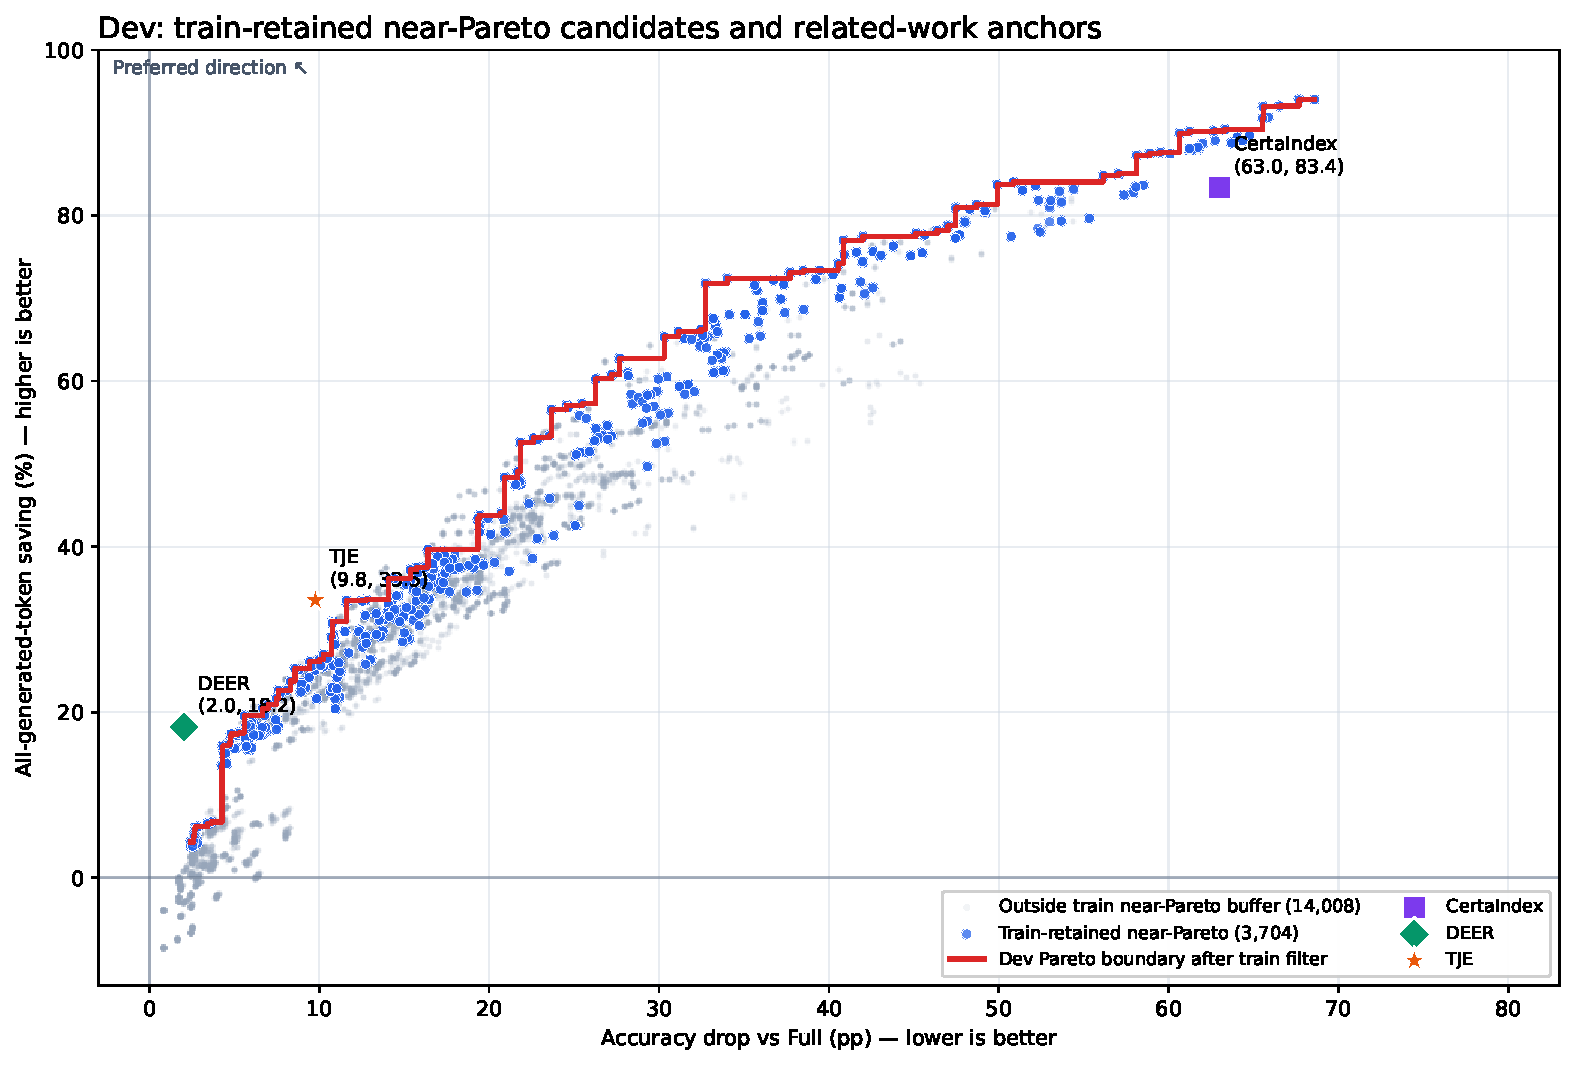
\includegraphics[width=\textwidth]{figures/governor_related_work_pareto_dev.pdf}
  \caption{\textbf{The safe-and-saving corner is empty.} Each grey point is one
  of the $17{,}712$ preregistered consensus rules on the development set; blue
  are the $3{,}704$ surviving a near-Pareto train filter, and the red step is the
  dev Pareto boundary. The top-left corner (small accuracy drop \emph{and} large
  token saving) contains no rule---the boundary only climbs as the drop grows.
  \textbf{CertaIndex} \citep{dynasor_certaindex}, the published consensus method,
  sits at the far right ($63\pp$ drop), the consensus family's collapse.
  \textbf{DEER} \citep{deer}, which reads a boundary-confidence signal
  \emph{outside} the swept space, occupies the low-drop corner
  ($2.0\pp$, $18\%$), above the consensus boundary at the same accuracy drop.
  The failure is a property of the consensus signal, not of early exit.}
  \label{fig:pareto}
\end{figure*}

\paragraph{Contribution.}
Our contribution is a rigorous, mechanism-backed demonstration that
\emph{intermediate answer-consensus is an unsafe early-exit signal for reasoning
LLMs}, established so that it cannot be waved away as an untuned heuristic. Three
components support this one claim:
\begin{itemize}
  \item \textbf{A preregistered, probe-independent test} (frozen trajectories,
  offline re-probing, a seven-dimensional $17{,}712$-rule schema, and selection
  gates fixed in advance) under which \emph{no} rule is both safe and
  token-saving---and which we release in full
  (Sections~\ref{sec:method}--\ref{sec:results}).
  \item \textbf{A mechanism} that explains \emph{why}: a directional
  ``continued-reasoning-corrects'' effect ($\approx\!35{:}1$) makes the accuracy
  cost of stopping intrinsic to the trajectory and independent of probe density,
  so the negative result generalizes beyond the searched schema
  (Section~\ref{sec:mechanism}).
  \item \textbf{Out-of-distribution and real-method confirmation}: the frontier
  reproduces on a held-out split and two unseen models, a published Certaindex
  reproduction collapses, and a non-consensus signal stays near full accuracy on
  the same trajectories---localizing the failure to consensus and indicating
  where a safe signal must come from (Sections~\ref{sec:results}--\ref{sec:mechanism}).
\end{itemize}
